% Options for packages loaded elsewhere
\PassOptionsToPackage{unicode}{hyperref}
\PassOptionsToPackage{hyphens}{url}
%
\documentclass[
]{article}
\usepackage{amsmath,amssymb}
\usepackage{iftex}
\ifPDFTeX
  \usepackage[T1]{fontenc}
  \usepackage[utf8]{inputenc}
  \usepackage{textcomp} % provide euro and other symbols
\else % if luatex or xetex
  \usepackage{unicode-math} % this also loads fontspec
  \defaultfontfeatures{Scale=MatchLowercase}
  \defaultfontfeatures[\rmfamily]{Ligatures=TeX,Scale=1}
\fi
\usepackage{lmodern}
\ifPDFTeX\else
  % xetex/luatex font selection
\fi
% Use upquote if available, for straight quotes in verbatim environments
\IfFileExists{upquote.sty}{\usepackage{upquote}}{}
\IfFileExists{microtype.sty}{% use microtype if available
  \usepackage[]{microtype}
  \UseMicrotypeSet[protrusion]{basicmath} % disable protrusion for tt fonts
}{}
\makeatletter
\@ifundefined{KOMAClassName}{% if non-KOMA class
  \IfFileExists{parskip.sty}{%
    \usepackage{parskip}
  }{% else
    \setlength{\parindent}{0pt}
    \setlength{\parskip}{6pt plus 2pt minus 1pt}}
}{% if KOMA class
  \KOMAoptions{parskip=half}}
\makeatother
\usepackage{xcolor}
\usepackage[margin=1in]{geometry}
\usepackage{color}
\usepackage{fancyvrb}
\newcommand{\VerbBar}{|}
\newcommand{\VERB}{\Verb[commandchars=\\\{\}]}
\DefineVerbatimEnvironment{Highlighting}{Verbatim}{commandchars=\\\{\}}
% Add ',fontsize=\small' for more characters per line
\usepackage{framed}
\definecolor{shadecolor}{RGB}{248,248,248}
\newenvironment{Shaded}{\begin{snugshade}}{\end{snugshade}}
\newcommand{\AlertTok}[1]{\textcolor[rgb]{0.94,0.16,0.16}{#1}}
\newcommand{\AnnotationTok}[1]{\textcolor[rgb]{0.56,0.35,0.01}{\textbf{\textit{#1}}}}
\newcommand{\AttributeTok}[1]{\textcolor[rgb]{0.13,0.29,0.53}{#1}}
\newcommand{\BaseNTok}[1]{\textcolor[rgb]{0.00,0.00,0.81}{#1}}
\newcommand{\BuiltInTok}[1]{#1}
\newcommand{\CharTok}[1]{\textcolor[rgb]{0.31,0.60,0.02}{#1}}
\newcommand{\CommentTok}[1]{\textcolor[rgb]{0.56,0.35,0.01}{\textit{#1}}}
\newcommand{\CommentVarTok}[1]{\textcolor[rgb]{0.56,0.35,0.01}{\textbf{\textit{#1}}}}
\newcommand{\ConstantTok}[1]{\textcolor[rgb]{0.56,0.35,0.01}{#1}}
\newcommand{\ControlFlowTok}[1]{\textcolor[rgb]{0.13,0.29,0.53}{\textbf{#1}}}
\newcommand{\DataTypeTok}[1]{\textcolor[rgb]{0.13,0.29,0.53}{#1}}
\newcommand{\DecValTok}[1]{\textcolor[rgb]{0.00,0.00,0.81}{#1}}
\newcommand{\DocumentationTok}[1]{\textcolor[rgb]{0.56,0.35,0.01}{\textbf{\textit{#1}}}}
\newcommand{\ErrorTok}[1]{\textcolor[rgb]{0.64,0.00,0.00}{\textbf{#1}}}
\newcommand{\ExtensionTok}[1]{#1}
\newcommand{\FloatTok}[1]{\textcolor[rgb]{0.00,0.00,0.81}{#1}}
\newcommand{\FunctionTok}[1]{\textcolor[rgb]{0.13,0.29,0.53}{\textbf{#1}}}
\newcommand{\ImportTok}[1]{#1}
\newcommand{\InformationTok}[1]{\textcolor[rgb]{0.56,0.35,0.01}{\textbf{\textit{#1}}}}
\newcommand{\KeywordTok}[1]{\textcolor[rgb]{0.13,0.29,0.53}{\textbf{#1}}}
\newcommand{\NormalTok}[1]{#1}
\newcommand{\OperatorTok}[1]{\textcolor[rgb]{0.81,0.36,0.00}{\textbf{#1}}}
\newcommand{\OtherTok}[1]{\textcolor[rgb]{0.56,0.35,0.01}{#1}}
\newcommand{\PreprocessorTok}[1]{\textcolor[rgb]{0.56,0.35,0.01}{\textit{#1}}}
\newcommand{\RegionMarkerTok}[1]{#1}
\newcommand{\SpecialCharTok}[1]{\textcolor[rgb]{0.81,0.36,0.00}{\textbf{#1}}}
\newcommand{\SpecialStringTok}[1]{\textcolor[rgb]{0.31,0.60,0.02}{#1}}
\newcommand{\StringTok}[1]{\textcolor[rgb]{0.31,0.60,0.02}{#1}}
\newcommand{\VariableTok}[1]{\textcolor[rgb]{0.00,0.00,0.00}{#1}}
\newcommand{\VerbatimStringTok}[1]{\textcolor[rgb]{0.31,0.60,0.02}{#1}}
\newcommand{\WarningTok}[1]{\textcolor[rgb]{0.56,0.35,0.01}{\textbf{\textit{#1}}}}
\usepackage{graphicx}
\makeatletter
\def\maxwidth{\ifdim\Gin@nat@width>\linewidth\linewidth\else\Gin@nat@width\fi}
\def\maxheight{\ifdim\Gin@nat@height>\textheight\textheight\else\Gin@nat@height\fi}
\makeatother
% Scale images if necessary, so that they will not overflow the page
% margins by default, and it is still possible to overwrite the defaults
% using explicit options in \includegraphics[width, height, ...]{}
\setkeys{Gin}{width=\maxwidth,height=\maxheight,keepaspectratio}
% Set default figure placement to htbp
\makeatletter
\def\fps@figure{htbp}
\makeatother
\setlength{\emergencystretch}{3em} % prevent overfull lines
\providecommand{\tightlist}{%
  \setlength{\itemsep}{0pt}\setlength{\parskip}{0pt}}
\setcounter{secnumdepth}{-\maxdimen} % remove section numbering
\renewcommand{\figurename}{Figure S}
\makeatletter
\def\fnum@figure{\figurename\thefigure}
\makeatother
\ifLuaTeX
  \usepackage{selnolig}  % disable illegal ligatures
\fi
\usepackage{bookmark}
\IfFileExists{xurl.sty}{\usepackage{xurl}}{} % add URL line breaks if available
\urlstyle{same}
\hypersetup{
  pdftitle={Supplementary material to: A detailed streamflow and groundwater salinity dataset for Muttama Creek Catchment, NSW, Australia - Manual adjustments groundwater standing waterlevels},
  hidelinks,
  pdfcreator={LaTeX via pandoc}}

\title{Supplementary material to: A detailed streamflow and groundwater
salinity dataset for Muttama Creek Catchment, NSW, Australia - Manual
adjustments groundwater standing waterlevels}
\author{}
\date{\vspace{-2.5em}2025-08-14}

\begin{document}
\maketitle

\subsection{Introduction}\label{introduction}

This workflow and data provenance description is related to the
groundwater level dataset in: ``A detailed streamflow and groundwater
salinity dataset for Muttama Creek Catchment, NSW, Australia'',
submitted to ESSD.

Automated scripts (\emph{SummariseDailyData.R} and
\emph{Match\_obs\_logger\_data.R}) have summarised the data to daily
values, adjusted logger values for the depth of measurement and adjusted
values based on the available manual observations.

The following pseudo code describes the matching between the raw logger
data and the manual observed data.

\begin{algorithm}
\caption{Pseudo code cleaning groundwater level data}
\label{pseudocode}
\begin{algorithmic}
\IF {sufficient points > 3} 
        \STATE run a regression between interpolated depth and observed depth  
        \STATE check the p-values of the slope and intercept
        \IF {the slope is not significant (using p > 0.10)}
                \STATE  use only the intercept to correct the logger data
        \ELSE
                \IF {the intercept is not significant, but the slope is}
                        \STATE use only the slope to correct the logger data
                \ELSE
                       \STATE use both slope and intercept of the regression to correct the logger data
                \ENDIF
        \ENDIF
\ELSE
        \STATE There are not enough values for a regression, use mean difference between logged and observed value to correct the logger data
\ENDIF
\end{algorithmic}
\end{algorithm}

The raw data and the scripts are documented on the associated OSF
project: \url{https://doi.org/10.17605/OSF.IO/BEUWK}. Here, only the
daily data resulting from this earlier data management are used.

\begin{figure}
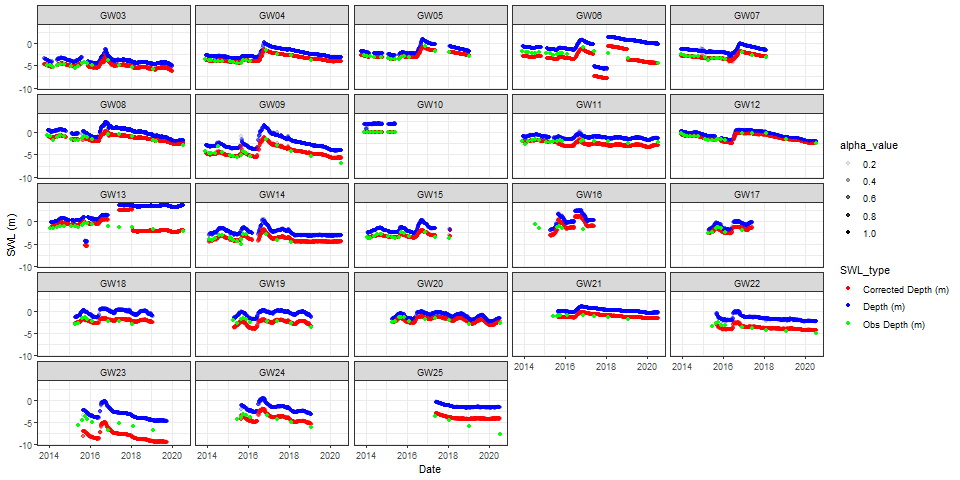
\includegraphics[width=0.95\linewidth]{../Figures/Corrected_piezodepths} \caption{Groundwater level logger data corrected for cable length and automatically matched to observed data.}\label{fig:piezodata}
\end{figure}

However, even after these adjustments, there are remaining anomalies in
some of the logger timeseries that can only be manually adjusted (Figure
\ref{fig:piezodata}). In particular, the loggers GW06 and GW13 show a
mismatch between observed data and logger data, or show strange jumps in
the logger data that clearly do not reflect groundwater behaviour.

The reasons for these differences can be unrecorded or lost recordings
of adjustments to the logger cable. There is a note that suggest an
adjustment to the GW06 and GW13 logger cables, but these don't fully
explain the observed anomalies.

As the scripts and automatic adjustments have not been able to remove
these anomalies, further adjustments can only be made manually. To
properly provide a provenance of these adjustments in the final data
set, this document records all the manual adjustments and the reasoning
behind those adjustments.

\subsection{Method}\label{method}

\begin{enumerate}
\def\labelenumi{\arabic{enumi}.}
\tightlist
\item
  load the R packages tidyverse and lubridate
\end{enumerate}

\begin{Shaded}
\begin{Highlighting}[]
\FunctionTok{require}\NormalTok{(tidyverse)}
\end{Highlighting}
\end{Shaded}

\begin{enumerate}
\def\labelenumi{\arabic{enumi}.}
\setcounter{enumi}{1}
\tightlist
\item
  read in the resulting data from the past analyses (i.e.~the data shown
  in Figure \ref{fig:piezodata}).
\end{enumerate}

\begin{Shaded}
\begin{Highlighting}[]
\NormalTok{GW\_data }\OtherTok{\textless{}{-}} \FunctionTok{read\_csv}\NormalTok{(}\StringTok{"../Data/CorrectedPiezoObservations.csv"}\NormalTok{)}
\end{Highlighting}
\end{Shaded}

\begin{verbatim}
## Rows: 36506 Columns: 11
## -- Column specification --------------------------------------------------------
## Delimiter: ","
## chr  (5): Piezo, type.x, Site, type.y, type
## dbl  (5): Obs Depth (m), Depth (m), SN, Int_depth, Corrected Depth (m)
## date (1): Date
## 
## i Use `spec()` to retrieve the full column specification for this data.
## i Specify the column types or set `show_col_types = FALSE` to quiet this message.
\end{verbatim}

\subsection{GW06}\label{gw06}

Filter out the data for the specific well

\begin{Shaded}
\begin{Highlighting}[]
\NormalTok{GW06 }\OtherTok{\textless{}{-}}\NormalTok{ GW\_data }\SpecialCharTok{\%\textgreater{}\%}
  \FunctionTok{filter}\NormalTok{(Piezo }\SpecialCharTok{==} \StringTok{"GW06"}\NormalTok{)}
\end{Highlighting}
\end{Shaded}

Identify jumps in the data using diff()

\begin{Shaded}
\begin{Highlighting}[]
\NormalTok{GW06 }\OtherTok{\textless{}{-}}\NormalTok{ GW06 }\SpecialCharTok{\%\textgreater{}\%}
  \FunctionTok{mutate}\NormalTok{(}\AttributeTok{diff\_gw =} \FunctionTok{c}\NormalTok{(}\DecValTok{0}\NormalTok{,}\FunctionTok{diff}\NormalTok{(GW06}\SpecialCharTok{$}\StringTok{\textasciigrave{}}\AttributeTok{Corrected Depth (m)}\StringTok{\textasciigrave{}}\NormalTok{)))}


\FunctionTok{png}\NormalTok{(}\StringTok{"../figures/HistogramGW06\_difference.png"}\NormalTok{)}
\FunctionTok{hist}\NormalTok{(GW06}\SpecialCharTok{$}\NormalTok{diff\_gw)}
\FunctionTok{dev.off}\NormalTok{()}
\end{Highlighting}
\end{Shaded}

\begin{verbatim}
## pdf 
##   2
\end{verbatim}

\begin{figure}
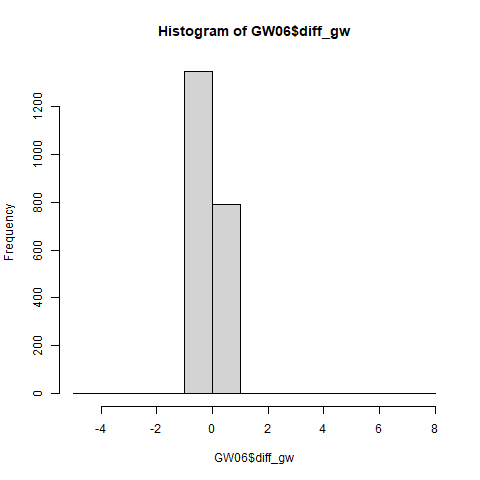
\includegraphics[width=0.8\linewidth]{../Figures/HistogramGW06_difference} \caption{Histogram of the jumps in the GW06 differenced data}\label{fig:hist-jumps-GW06}
\end{figure}

This indicates that any values \textgreater{} 2 and \textless{} -2 are
the anomalies. We can find the points where this transitions and then
find the values.

\begin{Shaded}
\begin{Highlighting}[]
\NormalTok{Dates }\OtherTok{\textless{}{-}}\NormalTok{ GW06 }\SpecialCharTok{\%\textgreater{}\%}
  \FunctionTok{filter}\NormalTok{(}\FunctionTok{abs}\NormalTok{(diff\_gw) }\SpecialCharTok{\textgreater{}} \DecValTok{2}\NormalTok{)}
\NormalTok{Dates}
\end{Highlighting}
\end{Shaded}

\begin{verbatim}
## # A tibble: 3 x 12
##   Date       `Obs Depth (m)` Piezo type.x `Depth (m)` Site         type.y     SN
##   <date>               <dbl> <chr> <chr>        <dbl> <chr>        <chr>   <dbl>
## 1 2017-06-05              NA GW06  <NA>        -5.21  Brawlin Spr~ Logger 1.07e6
## 2 2018-02-05              NA GW06  <NA>         1.42  Brawlin Spr~ Logger 1.07e6
## 3 2019-01-29              NA GW06  <NA>         0.671 Brawlin Spr~ Logger 1.06e6
## # i 4 more variables: Int_depth <dbl>, `Corrected Depth (m)` <dbl>, type <chr>,
## #   diff_gw <dbl>
\end{verbatim}

Comparing Figure \ref{fig:hist-jumps-GW06} to Figure
\ref{fig:piezodata}, this means the section between 2017-06-05 and
2018-02-05 needs to be corrected by -4.9065 being the difference in the
anomaly (bias) at the beginning of the section. This value is close to
the adjustment value in the field notes of 4.95m on \emph{2017-06-02}
which is also close to 2017-06-05. The section past 2018-02-05 until
2019-01-29 needs to be corrected by -2.326666 which is the estimate of
the positive bias at the end. This value differs from the earlier
correction and it is unclear where this difference comes from.

\begin{Shaded}
\begin{Highlighting}[]
\CommentTok{\# correction for the first section}
\NormalTok{correction1 }\OtherTok{\textless{}{-}}\NormalTok{ Dates}\SpecialCharTok{$}\NormalTok{diff\_gw[}\DecValTok{1}\NormalTok{]}
\CommentTok{\# correction for the second section}
\NormalTok{correction2 }\OtherTok{\textless{}{-}}\NormalTok{ Dates}\SpecialCharTok{$}\NormalTok{diff\_gw[}\DecValTok{3}\NormalTok{]}
\NormalTok{GW06 }\OtherTok{\textless{}{-}}\NormalTok{ GW06 }\SpecialCharTok{\%\textgreater{}\%}
  \FunctionTok{mutate}\NormalTok{(}\StringTok{\textasciigrave{}}\AttributeTok{Manual correct}\StringTok{\textasciigrave{}} \OtherTok{=} \FunctionTok{ifelse}\NormalTok{(GW06}\SpecialCharTok{$}\NormalTok{Date }\SpecialCharTok{\textgreater{}=}\NormalTok{ Dates}\SpecialCharTok{$}\NormalTok{Date[}\DecValTok{1}\NormalTok{] }\SpecialCharTok{\&}
\NormalTok{                                     GW06}\SpecialCharTok{$}\NormalTok{Date }\SpecialCharTok{\textless{}}\NormalTok{ Dates}\SpecialCharTok{$}\NormalTok{Date[}\DecValTok{2}\NormalTok{],}
                                   \StringTok{\textasciigrave{}}\AttributeTok{Corrected Depth (m)}\StringTok{\textasciigrave{}} \SpecialCharTok{{-}}
\NormalTok{                                     correction1,}
                                   \StringTok{\textasciigrave{}}\AttributeTok{Corrected Depth (m)}\StringTok{\textasciigrave{}}\NormalTok{)) }\SpecialCharTok{\%\textgreater{}\%}
  \FunctionTok{mutate}\NormalTok{(}\AttributeTok{Ind =} \FunctionTok{ifelse}\NormalTok{(GW06}\SpecialCharTok{$}\NormalTok{Date }\SpecialCharTok{\textgreater{}=}\NormalTok{ Dates}\SpecialCharTok{$}\NormalTok{Date[}\DecValTok{1}\NormalTok{] }\SpecialCharTok{\&}
\NormalTok{                                     GW06}\SpecialCharTok{$}\NormalTok{Date }\SpecialCharTok{\textless{}}\NormalTok{ Dates}\SpecialCharTok{$}\NormalTok{Date[}\DecValTok{2}\NormalTok{],}\DecValTok{1}\NormalTok{,}\DecValTok{0}\NormalTok{))}

\NormalTok{GW06 }\OtherTok{\textless{}{-}}\NormalTok{ GW06 }\SpecialCharTok{\%\textgreater{}\%}
  \FunctionTok{mutate}\NormalTok{(}\StringTok{\textasciigrave{}}\AttributeTok{Manual correct}\StringTok{\textasciigrave{}} \OtherTok{=} \FunctionTok{ifelse}\NormalTok{(GW06}\SpecialCharTok{$}\NormalTok{Date }\SpecialCharTok{\textgreater{}=}\NormalTok{ Dates}\SpecialCharTok{$}\NormalTok{Date[}\DecValTok{2}\NormalTok{] }\SpecialCharTok{\&}
\NormalTok{                                     GW06}\SpecialCharTok{$}\NormalTok{Date }\SpecialCharTok{\textless{}=}\NormalTok{ Dates}\SpecialCharTok{$}\NormalTok{Date[}\DecValTok{3}\NormalTok{]}\SpecialCharTok{+}\DecValTok{1}\NormalTok{,}
                                   \StringTok{\textasciigrave{}}\AttributeTok{Manual correct}\StringTok{\textasciigrave{}} \SpecialCharTok{+}
\NormalTok{                                     correction2,}
                                   \StringTok{\textasciigrave{}}\AttributeTok{Manual correct}\StringTok{\textasciigrave{}}\NormalTok{)) }\SpecialCharTok{\%\textgreater{}\%}
  \FunctionTok{mutate}\NormalTok{(}\AttributeTok{Ind =} \FunctionTok{ifelse}\NormalTok{(GW06}\SpecialCharTok{$}\NormalTok{Date }\SpecialCharTok{\textgreater{}=}\NormalTok{ Dates}\SpecialCharTok{$}\NormalTok{Date[}\DecValTok{2}\NormalTok{] }\SpecialCharTok{\&}
\NormalTok{                                     GW06}\SpecialCharTok{$}\NormalTok{Date }\SpecialCharTok{\textless{}=}\NormalTok{ Dates}\SpecialCharTok{$}\NormalTok{Date[}\DecValTok{3}\NormalTok{]}\SpecialCharTok{+}\DecValTok{1}\NormalTok{,}\DecValTok{1}\NormalTok{,Ind))}

\FunctionTok{png}\NormalTok{(}\StringTok{"../Figures/GW06\_firstcorrection.png"}\NormalTok{)}
\NormalTok{GW06 }\SpecialCharTok{\%\textgreater{}\%}
  \FunctionTok{ggplot}\NormalTok{(}\FunctionTok{aes}\NormalTok{(Date,}\StringTok{\textasciigrave{}}\AttributeTok{Corrected Depth (m)}\StringTok{\textasciigrave{}}\NormalTok{)) }\SpecialCharTok{+} 
  \FunctionTok{geom\_point}\NormalTok{(}\AttributeTok{colour =} \StringTok{"blue"}\NormalTok{) }\SpecialCharTok{+}
  \FunctionTok{geom\_point}\NormalTok{(}\FunctionTok{aes}\NormalTok{(Date,}\StringTok{\textasciigrave{}}\AttributeTok{Manual correct}\StringTok{\textasciigrave{}}\NormalTok{),}\AttributeTok{colour =} \StringTok{"red"}\NormalTok{)}
\end{Highlighting}
\end{Shaded}

\begin{verbatim}
## Warning: Removed 18 rows containing missing values or values outside the scale range
## (`geom_point()`).
## Removed 18 rows containing missing values or values outside the scale range
## (`geom_point()`).
\end{verbatim}

\begin{Shaded}
\begin{Highlighting}[]
\FunctionTok{dev.off}\NormalTok{()}
\end{Highlighting}
\end{Shaded}

\begin{verbatim}
## pdf 
##   2
\end{verbatim}

\begin{figure}
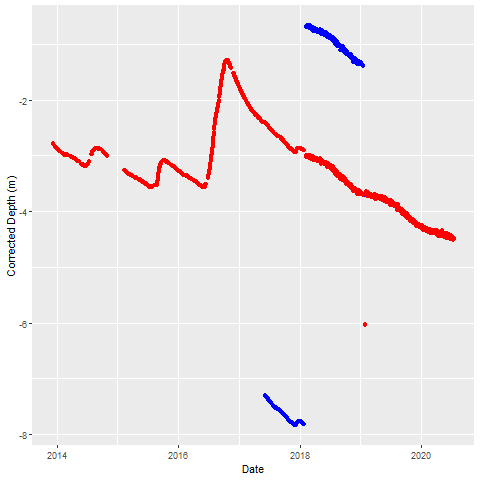
\includegraphics[width=0.8\linewidth]{../Figures/GW06_firstcorrection} \caption{First correction of the GW06 groundwater level data}\label{fig:firstcorr-GW06}
\end{figure}

This appears to require one further correction,to removes the single
anomaly in 2019.

\begin{Shaded}
\begin{Highlighting}[]
\CommentTok{\# recalculate diff, but now based on manual correct}
\NormalTok{GW06 }\OtherTok{\textless{}{-}}\NormalTok{ GW06 }\SpecialCharTok{\%\textgreater{}\%}
  \FunctionTok{mutate}\NormalTok{(}\AttributeTok{diff\_gw =} \FunctionTok{c}\NormalTok{(}\DecValTok{0}\NormalTok{,}\FunctionTok{diff}\NormalTok{(GW06}\SpecialCharTok{$}\StringTok{\textasciigrave{}}\AttributeTok{Manual correct}\StringTok{\textasciigrave{}}\NormalTok{)))}

\NormalTok{Dates }\OtherTok{\textless{}{-}}\NormalTok{ GW06 }\SpecialCharTok{\%\textgreater{}\%}
  \FunctionTok{filter}\NormalTok{(}\FunctionTok{abs}\NormalTok{(diff\_gw) }\SpecialCharTok{\textgreater{}} \FloatTok{1.5}\NormalTok{)}
\NormalTok{Dates}
\end{Highlighting}
\end{Shaded}

\begin{verbatim}
## # A tibble: 2 x 14
##   Date       `Obs Depth (m)` Piezo type.x `Depth (m)` Site         type.y     SN
##   <date>               <dbl> <chr> <chr>        <dbl> <chr>        <chr>   <dbl>
## 1 2019-01-29              NA GW06  <NA>         0.671 Brawlin Spr~ Logger 1.06e6
## 2 2019-01-31              NA GW06  <NA>         0.700 Brawlin Spr~ Logger 1.06e6
## # i 6 more variables: Int_depth <dbl>, `Corrected Depth (m)` <dbl>, type <chr>,
## #   diff_gw <dbl>, `Manual correct` <dbl>, Ind <dbl>
\end{verbatim}

\begin{Shaded}
\begin{Highlighting}[]
\NormalTok{correction3 }\OtherTok{\textless{}{-}}\NormalTok{ Dates}\SpecialCharTok{$}\NormalTok{diff\_gw[}\DecValTok{1}\NormalTok{]}

\CommentTok{\# GW06 \textless{}{-} GW06 \%\textgreater{}\%}
\CommentTok{\#   mutate(\textasciigrave{}Manual correct\textasciigrave{} = ifelse(GW06$Date \textgreater{}= Dates$Date[1],}
\CommentTok{\#                                    \textasciigrave{}Manual correct\textasciigrave{} {-}}
\CommentTok{\#                                      correction3,}
\CommentTok{\#                                    \textasciigrave{}Manual correct\textasciigrave{}))}
\CommentTok{\#delete final point}
\NormalTok{GW06 }\OtherTok{\textless{}{-}}\NormalTok{ GW06 }\SpecialCharTok{\%\textgreater{}\%} 
  \FunctionTok{mutate}\NormalTok{(}\StringTok{\textasciigrave{}}\AttributeTok{Manual correct}\StringTok{\textasciigrave{}} \OtherTok{=} \FunctionTok{ifelse}\NormalTok{(GW06}\SpecialCharTok{$}\NormalTok{Date }\SpecialCharTok{\textgreater{}=}\NormalTok{ Dates}\SpecialCharTok{$}\NormalTok{Date[}\DecValTok{1}\NormalTok{] }\SpecialCharTok{\&}
\NormalTok{                                     GW06}\SpecialCharTok{$}\NormalTok{Date }\SpecialCharTok{\textless{}=}\NormalTok{ Dates}\SpecialCharTok{$}\NormalTok{Date[}\DecValTok{2}\NormalTok{],}
                                   \ConstantTok{NA}\NormalTok{,}
                                   \StringTok{\textasciigrave{}}\AttributeTok{Manual correct}\StringTok{\textasciigrave{}}\NormalTok{)) }\SpecialCharTok{\%\textgreater{}\%}
  \FunctionTok{mutate}\NormalTok{(}\AttributeTok{Ind =} \FunctionTok{ifelse}\NormalTok{(GW06}\SpecialCharTok{$}\NormalTok{Date }\SpecialCharTok{\textgreater{}=}\NormalTok{ Dates}\SpecialCharTok{$}\NormalTok{Date[}\DecValTok{1}\NormalTok{] }\SpecialCharTok{\&}
\NormalTok{                                     GW06}\SpecialCharTok{$}\NormalTok{Date }\SpecialCharTok{\textless{}=}\NormalTok{ Dates}\SpecialCharTok{$}\NormalTok{Date[}\DecValTok{2}\NormalTok{],}\DecValTok{1}\NormalTok{,Ind))}

\FunctionTok{png}\NormalTok{(}\StringTok{"../Figures/GW06\_secondcorrection.png"}\NormalTok{)}
\NormalTok{GW06 }\SpecialCharTok{\%\textgreater{}\%}
  \FunctionTok{ggplot}\NormalTok{(}\FunctionTok{aes}\NormalTok{(Date,}\StringTok{\textasciigrave{}}\AttributeTok{Corrected Depth (m)}\StringTok{\textasciigrave{}}\NormalTok{)) }\SpecialCharTok{+} 
  \FunctionTok{geom\_point}\NormalTok{(}\AttributeTok{colour =} \StringTok{"blue"}\NormalTok{) }\SpecialCharTok{+}
  \FunctionTok{geom\_point}\NormalTok{(}\FunctionTok{aes}\NormalTok{(Date,}\StringTok{\textasciigrave{}}\AttributeTok{Manual correct}\StringTok{\textasciigrave{}}\NormalTok{),}\AttributeTok{colour =} \StringTok{"red"}\NormalTok{)}
\end{Highlighting}
\end{Shaded}

\begin{verbatim}
## Warning: Removed 18 rows containing missing values or values outside the scale range
## (`geom_point()`).
\end{verbatim}

\begin{verbatim}
## Warning: Removed 21 rows containing missing values or values outside the scale range
## (`geom_point()`).
\end{verbatim}

\begin{Shaded}
\begin{Highlighting}[]
\FunctionTok{dev.off}\NormalTok{()}
\end{Highlighting}
\end{Shaded}

\begin{verbatim}
## pdf 
##   2
\end{verbatim}

\begin{figure}
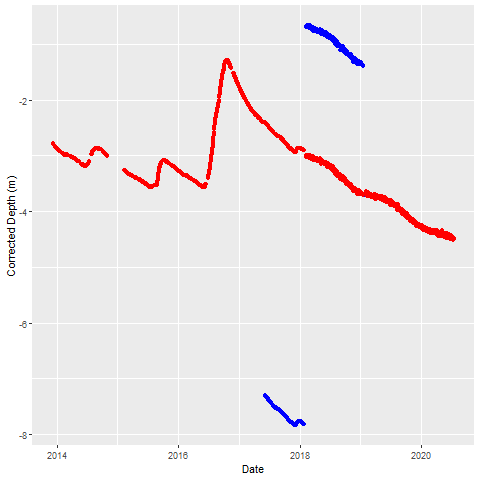
\includegraphics[width=0.8\linewidth]{../Figures/GW06_secondcorrection} \caption{Second correction of the GW06 groundwater level data}\label{fig:secondcorr-GW06}
\end{figure}

Finally, we can clean up so we only retain the ``Manual correct''
column, but none of the intermediate columns.

\subsection{GW13}\label{gw13}

Essentially we will use the same process.

Filter out the data for the specific well

\begin{Shaded}
\begin{Highlighting}[]
\NormalTok{GW13 }\OtherTok{\textless{}{-}}\NormalTok{ GW\_data }\SpecialCharTok{\%\textgreater{}\%}
  \FunctionTok{filter}\NormalTok{(Piezo }\SpecialCharTok{==} \StringTok{"GW13"}\NormalTok{)}
\end{Highlighting}
\end{Shaded}

Directly identifying jumps in the data using diff() does not work in
this case due to missing data in the corrected depth data. so this needs
to be filtered first, before calculating the \texttt{diff()} values

\begin{Shaded}
\begin{Highlighting}[]
\NormalTok{GW13\_noNA }\OtherTok{\textless{}{-}}\NormalTok{ GW13 }\SpecialCharTok{\%\textgreater{}\%}
  \CommentTok{\#filter(is.na(\textasciigrave{}Corrected Depth (m)\textasciigrave{}) == F) \%\textgreater{}\%}
  \FunctionTok{mutate}\NormalTok{(}\AttributeTok{diff\_gw =} \FunctionTok{c}\NormalTok{(}\DecValTok{0}\NormalTok{,}\FunctionTok{diff}\NormalTok{(}\StringTok{\textasciigrave{}}\AttributeTok{Corrected Depth (m)}\StringTok{\textasciigrave{}}\NormalTok{)))}

\FunctionTok{png}\NormalTok{(}\StringTok{"../figures/HistogramGW13\_difference.png"}\NormalTok{)}
\FunctionTok{hist}\NormalTok{(GW13\_noNA}\SpecialCharTok{$}\NormalTok{diff\_gw)}
\FunctionTok{dev.off}\NormalTok{()}
\end{Highlighting}
\end{Shaded}

\begin{verbatim}
## pdf 
##   2
\end{verbatim}

\begin{figure}
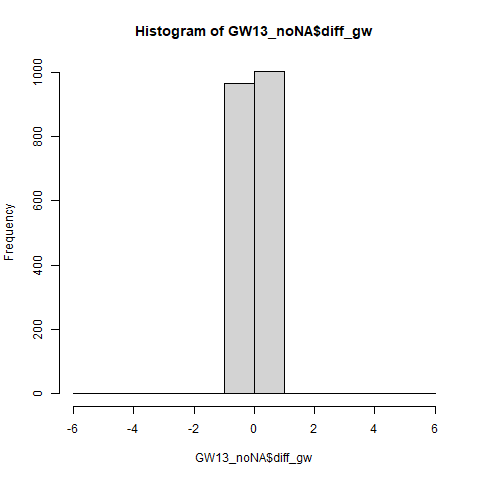
\includegraphics[width=0.8\linewidth]{../Figures/HistogramGW13_difference} \caption{Histogram of the jumps in the GW13 differenced data}\label{fig:hist-jumps-GW13}
\end{figure}

Figure \ref{fig:hist-jumps-GW13} indicates that any values
\textgreater{} 1 and \textless{} -1 are the anomalies. We can find the
points where this transitions and then find the dates.

\begin{Shaded}
\begin{Highlighting}[]
\NormalTok{Dates }\OtherTok{\textless{}{-}}\NormalTok{ GW13\_noNA }\SpecialCharTok{\%\textgreater{}\%}
  \FunctionTok{filter}\NormalTok{(}\FunctionTok{abs}\NormalTok{(diff\_gw) }\SpecialCharTok{\textgreater{}} \DecValTok{1}\NormalTok{) }\SpecialCharTok{\%\textgreater{}\%}
  \FunctionTok{arrange}\NormalTok{(Date)}
\NormalTok{Dates }\SpecialCharTok{\%\textgreater{}\%}
\NormalTok{  dplyr}\SpecialCharTok{::}\FunctionTok{select}\NormalTok{(Date,diff\_gw)}
\end{Highlighting}
\end{Shaded}

\begin{verbatim}
## # A tibble: 5 x 2
##   Date       diff_gw
##   <date>       <dbl>
## 1 2015-10-03   -5.30
## 2 2015-11-24   -2.92
## 3 2016-02-15    5.13
## 4 2017-06-03    2.10
## 5 2018-02-05   -1.38
\end{verbatim}

Comparing Figure \ref{fig:hist-jumps-GW13} to Figure
\ref{fig:piezodata}, the first two dates relate to the small number of
anomalies earlier in the time series. This means the section between
2015-10-03 and 2015-11-24 needs to be corrected by -5.2971667 being the
difference in the anomaly (bias) at the beginning of the section.

The later section is trickier as the \texttt{diff()} results do not
identify the correct anomaly in the data (which should be around 4 m),
because of all the missing values in the data. The results from
\texttt{diff()} only finds 5.1299167 as the largest difference, but this
probably overdoes the correction.

\begin{Shaded}
\begin{Highlighting}[]
\CommentTok{\# correction for the first section}
\NormalTok{correction1 }\OtherTok{\textless{}{-}}\NormalTok{ Dates}\SpecialCharTok{$}\NormalTok{diff\_gw[}\DecValTok{1}\NormalTok{]}
\CommentTok{\# correction for the second section}
\NormalTok{correction2 }\OtherTok{\textless{}{-}}\NormalTok{ Dates}\SpecialCharTok{$}\NormalTok{diff\_gw[}\DecValTok{3}\NormalTok{] }
\NormalTok{GW13 }\OtherTok{\textless{}{-}}\NormalTok{ GW13 }\SpecialCharTok{\%\textgreater{}\%}
  \FunctionTok{mutate}\NormalTok{(}\StringTok{\textasciigrave{}}\AttributeTok{Manual correct}\StringTok{\textasciigrave{}} \OtherTok{=} \FunctionTok{ifelse}\NormalTok{(GW13}\SpecialCharTok{$}\NormalTok{Date }\SpecialCharTok{\textgreater{}=}\NormalTok{ Dates}\SpecialCharTok{$}\NormalTok{Date[}\DecValTok{1}\NormalTok{] }\SpecialCharTok{\&}
\NormalTok{                                     GW13}\SpecialCharTok{$}\NormalTok{Date }\SpecialCharTok{\textless{}}\NormalTok{ Dates}\SpecialCharTok{$}\NormalTok{Date[}\DecValTok{2}\NormalTok{],}
                                   \StringTok{\textasciigrave{}}\AttributeTok{Corrected Depth (m)}\StringTok{\textasciigrave{}} \SpecialCharTok{{-}}
\NormalTok{                                     correction1,}
                                   \StringTok{\textasciigrave{}}\AttributeTok{Corrected Depth (m)}\StringTok{\textasciigrave{}}\NormalTok{)) }\SpecialCharTok{\%\textgreater{}\%}
  \FunctionTok{mutate}\NormalTok{(}\StringTok{\textasciigrave{}}\AttributeTok{Manual correct}\StringTok{\textasciigrave{}} \OtherTok{=} \FunctionTok{ifelse}\NormalTok{(GW13}\SpecialCharTok{$}\NormalTok{Date }\SpecialCharTok{\textgreater{}=}
\NormalTok{                                     Dates}\SpecialCharTok{$}\NormalTok{Date[}\DecValTok{4}\NormalTok{] }\SpecialCharTok{\&}
\NormalTok{                                     GW13}\SpecialCharTok{$}\NormalTok{Date }\SpecialCharTok{\textless{}}
\NormalTok{                                     Dates}\SpecialCharTok{$}\NormalTok{Date[}\DecValTok{5}\NormalTok{],}
                                   \StringTok{\textasciigrave{}}\AttributeTok{Manual correct}\StringTok{\textasciigrave{}} \SpecialCharTok{{-}}
\NormalTok{                                     correction2,}
                                   \StringTok{\textasciigrave{}}\AttributeTok{Manual correct}\StringTok{\textasciigrave{}}\NormalTok{)) }\SpecialCharTok{\%\textgreater{}\%}
  \FunctionTok{mutate}\NormalTok{(}\AttributeTok{Ind =} \FunctionTok{ifelse}\NormalTok{(GW13}\SpecialCharTok{$}\NormalTok{Date }\SpecialCharTok{\textgreater{}=}\NormalTok{ Dates}\SpecialCharTok{$}\NormalTok{Date[}\DecValTok{1}\NormalTok{] }\SpecialCharTok{\&}
\NormalTok{                                     GW13}\SpecialCharTok{$}\NormalTok{Date }\SpecialCharTok{\textless{}}\NormalTok{ Dates}\SpecialCharTok{$}\NormalTok{Date[}\DecValTok{2}\NormalTok{],}\DecValTok{1}\NormalTok{,}\DecValTok{0}\NormalTok{)) }\SpecialCharTok{\%\textgreater{}\%}
  \FunctionTok{mutate}\NormalTok{(}\AttributeTok{Ind =} \FunctionTok{ifelse}\NormalTok{(GW13}\SpecialCharTok{$}\NormalTok{Date }\SpecialCharTok{\textgreater{}=}
\NormalTok{                                     Dates}\SpecialCharTok{$}\NormalTok{Date[}\DecValTok{4}\NormalTok{] }\SpecialCharTok{\&}
\NormalTok{                                     GW13}\SpecialCharTok{$}\NormalTok{Date }\SpecialCharTok{\textless{}}
\NormalTok{                                     Dates}\SpecialCharTok{$}\NormalTok{Date[}\DecValTok{5}\NormalTok{],}\DecValTok{1}\NormalTok{,Ind))}

\FunctionTok{png}\NormalTok{(}\StringTok{"../figures/Correction\_GW13.png"}\NormalTok{)}
\NormalTok{GW13 }\SpecialCharTok{\%\textgreater{}\%}
  \FunctionTok{pivot\_longer}\NormalTok{(}\FunctionTok{c}\NormalTok{(}\StringTok{\textasciigrave{}}\AttributeTok{Corrected Depth (m)}\StringTok{\textasciigrave{}}\NormalTok{,}\StringTok{\textasciigrave{}}\AttributeTok{Manual correct}\StringTok{\textasciigrave{}}\NormalTok{), }\AttributeTok{values\_to =} \StringTok{"Depth"}\NormalTok{,}
              \AttributeTok{names\_to =} \StringTok{"Method"}\NormalTok{) }\SpecialCharTok{\%\textgreater{}\%}
  \FunctionTok{ggplot}\NormalTok{(}\FunctionTok{aes}\NormalTok{(Date, Depth, }\AttributeTok{colour =}\NormalTok{ Method)) }\SpecialCharTok{+} \FunctionTok{geom\_point}\NormalTok{() }\SpecialCharTok{+}
  \FunctionTok{geom\_point}\NormalTok{(}\FunctionTok{aes}\NormalTok{(Date, Ind), }\AttributeTok{colour =} \StringTok{"yellow"}\NormalTok{) }\SpecialCharTok{+}
  \FunctionTok{scale\_colour\_manual}\NormalTok{(}\AttributeTok{values =} \FunctionTok{c}\NormalTok{(}\StringTok{"Corrected Depth (m)"} \OtherTok{=} \StringTok{"blue"}\NormalTok{, }\StringTok{"Manual correct"} \OtherTok{=} \StringTok{"red"}\NormalTok{))}
\end{Highlighting}
\end{Shaded}

\begin{verbatim}
## Warning: Removed 34 rows containing missing values or values outside the scale range
## (`geom_point()`).
\end{verbatim}

\begin{Shaded}
\begin{Highlighting}[]
\FunctionTok{dev.off}\NormalTok{()}
\end{Highlighting}
\end{Shaded}

\begin{verbatim}
## pdf 
##   2
\end{verbatim}

\begin{figure}
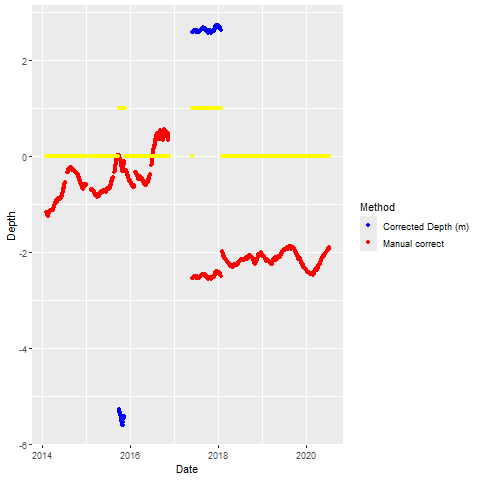
\includegraphics[width=0.8\linewidth]{../Figures/Correction_GW13} \caption{Correction of the GW13 groundwater level timeseries}\label{fig:corr-GW13}
\end{figure}

\subsection{producing the final
output}\label{producing-the-final-output}

Combine the manually corrected values into the original data, but save
this under a different file name. It is important to keep the different
corrected versions separate.

Add a column \texttt{Source} to indicate what version of the data the
final version is.

\begin{Shaded}
\begin{Highlighting}[]
\NormalTok{GW\_data\_output }\OtherTok{\textless{}{-}}\NormalTok{ GW\_data }\SpecialCharTok{\%\textgreater{}\%}
  \FunctionTok{mutate}\NormalTok{(}\StringTok{\textasciigrave{}}\AttributeTok{Final GW Depth (m)}\StringTok{\textasciigrave{}} \OtherTok{=} \StringTok{\textasciigrave{}}\AttributeTok{Corrected Depth (m)}\StringTok{\textasciigrave{}}\NormalTok{,}
         \AttributeTok{Source =} \StringTok{"Automatic correction"}\NormalTok{) }\SpecialCharTok{\%\textgreater{}\%}
  \FunctionTok{filter}\NormalTok{(Piezo }\SpecialCharTok{!=} \StringTok{\textquotesingle{}GW06\textquotesingle{}}\NormalTok{) }\SpecialCharTok{\%\textgreater{}\%}
  \FunctionTok{filter}\NormalTok{(Piezo }\SpecialCharTok{!=} \StringTok{\textquotesingle{}GW13\textquotesingle{}}\NormalTok{)}

\NormalTok{GW06\_f }\OtherTok{\textless{}{-}}\NormalTok{ GW06 }\SpecialCharTok{\%\textgreater{}\%}
  \FunctionTok{mutate}\NormalTok{(}\StringTok{\textasciigrave{}}\AttributeTok{Final GW Depth (m)}\StringTok{\textasciigrave{}} \OtherTok{=} \StringTok{\textasciigrave{}}\AttributeTok{Manual correct}\StringTok{\textasciigrave{}}\NormalTok{,}
         \AttributeTok{Source =} \FunctionTok{ifelse}\NormalTok{(Ind }\SpecialCharTok{==} \DecValTok{1}\NormalTok{,}
                         \StringTok{"Manual correction"}\NormalTok{,}\StringTok{\textquotesingle{}Automatic correction\textquotesingle{}}\NormalTok{)) }
\NormalTok{GW13\_f }\OtherTok{\textless{}{-}}\NormalTok{ GW13 }\SpecialCharTok{\%\textgreater{}\%}
  \FunctionTok{mutate}\NormalTok{(}\StringTok{\textasciigrave{}}\AttributeTok{Final GW Depth (m)}\StringTok{\textasciigrave{}} \OtherTok{=} \StringTok{\textasciigrave{}}\AttributeTok{Manual correct}\StringTok{\textasciigrave{}}\NormalTok{,}
         \AttributeTok{Source =} \FunctionTok{ifelse}\NormalTok{(Ind }\SpecialCharTok{==} \DecValTok{1}\NormalTok{,}
                         \StringTok{"Manual correction"}\NormalTok{,}\StringTok{\textquotesingle{}Automatic correction\textquotesingle{}}\NormalTok{)) }
         
\NormalTok{GW\_data\_output }\OtherTok{\textless{}{-}} \FunctionTok{bind\_rows}\NormalTok{(GW\_data\_output, GW06\_f, GW13\_f)  }
\end{Highlighting}
\end{Shaded}

Now delete any of the intermediary columns

\begin{Shaded}
\begin{Highlighting}[]
\FunctionTok{png}\NormalTok{(}\StringTok{"../Figures/Final\_Corrected\_piezodepths.png"}\NormalTok{, }\AttributeTok{width =} \DecValTok{1080}\NormalTok{, }\AttributeTok{height =} \DecValTok{760}\NormalTok{)}

\NormalTok{GW\_data\_output }\OtherTok{\textless{}{-}}\NormalTok{ GW\_data\_output }\SpecialCharTok{\%\textgreater{}\%}
\NormalTok{  dplyr}\SpecialCharTok{::}\FunctionTok{select}\NormalTok{(}\SpecialCharTok{{-}}\FunctionTok{c}\NormalTok{(}\StringTok{\textasciigrave{}}\AttributeTok{Depth (m)}\StringTok{\textasciigrave{}}\NormalTok{,}
\NormalTok{            type.x, type.y, type, Int\_depth))}
\NormalTok{GW\_data\_output }\SpecialCharTok{\%\textgreater{}\%}
  \FunctionTok{mutate}\NormalTok{(}\StringTok{\textasciigrave{}}\AttributeTok{Observed Depth (m)}\StringTok{\textasciigrave{}} \OtherTok{=} \StringTok{\textasciigrave{}}\AttributeTok{Obs Depth (m)}\StringTok{\textasciigrave{}}\NormalTok{) }\SpecialCharTok{\%\textgreater{}\%}
  \FunctionTok{pivot\_longer}\NormalTok{(}\AttributeTok{cols=}\FunctionTok{c}\NormalTok{(}\StringTok{\textasciigrave{}}\AttributeTok{Observed Depth (m)}\StringTok{\textasciigrave{}}\NormalTok{, }\StringTok{\textasciigrave{}}\AttributeTok{Final GW Depth (m)}\StringTok{\textasciigrave{}}\NormalTok{), }
               \AttributeTok{names\_to =} \StringTok{"SWL\_type"}\NormalTok{, }\AttributeTok{values\_to =} \StringTok{"SWL (m)"}\NormalTok{) }\SpecialCharTok{\%\textgreater{}\%} 
  \FunctionTok{mutate}\NormalTok{(}\AttributeTok{alpha\_value =} \FunctionTok{ifelse}\NormalTok{(SWL\_type }\SpecialCharTok{==} \StringTok{"Observed Depth (m)"}\NormalTok{,}\DecValTok{1}\NormalTok{,}\FloatTok{0.2}\NormalTok{),}
         \AttributeTok{Source =} \FunctionTok{ifelse}\NormalTok{(SWL\_type }\SpecialCharTok{==} \StringTok{"Observed Depth (m)"}\NormalTok{,}\StringTok{"Observed Depth (m)"}\NormalTok{,Source)) }\SpecialCharTok{\%\textgreater{}\%}
  \FunctionTok{ggplot}\NormalTok{(}\FunctionTok{aes}\NormalTok{(Date,}\StringTok{\textasciigrave{}}\AttributeTok{SWL (m)}\StringTok{\textasciigrave{}}\NormalTok{, }\AttributeTok{colour =}\NormalTok{ Source, }\AttributeTok{alpha =}\NormalTok{ alpha\_value)) }\SpecialCharTok{+} 
  \FunctionTok{geom\_point}\NormalTok{() }\SpecialCharTok{+} 
  \FunctionTok{facet\_wrap}\NormalTok{(}\SpecialCharTok{\textasciitilde{}}\NormalTok{Piezo, }\AttributeTok{ncol =} \DecValTok{4}\NormalTok{) }\SpecialCharTok{+} \FunctionTok{theme\_bw}\NormalTok{() }\SpecialCharTok{+} 
  \FunctionTok{scale\_color\_manual}\NormalTok{(}\AttributeTok{values=}\FunctionTok{c}\NormalTok{(}\StringTok{"Automatic correction"} \OtherTok{=} \StringTok{"\#E69F00"}\NormalTok{,}
                             \StringTok{"Manual correction"} \OtherTok{=} \StringTok{"\#56B4E9"}\NormalTok{ ,}
                             \StringTok{"Observed Depth (m)"} \OtherTok{=} \StringTok{"\#009E73"}\NormalTok{)) }\SpecialCharTok{+}
  \FunctionTok{theme}\NormalTok{(}\AttributeTok{axis.text =} \FunctionTok{element\_text}\NormalTok{(}\AttributeTok{size  =} \FunctionTok{rel}\NormalTok{(}\FloatTok{1.2}\NormalTok{)),}
        \AttributeTok{axis.title =} \FunctionTok{element\_text}\NormalTok{(}\AttributeTok{size =} \FunctionTok{rel}\NormalTok{(}\FloatTok{1.2}\NormalTok{)),}
        \AttributeTok{legend.text =} \FunctionTok{element\_text}\NormalTok{(}\AttributeTok{size  =} \FunctionTok{rel}\NormalTok{(}\FloatTok{1.2}\NormalTok{)),}
        \AttributeTok{legend.title =} \FunctionTok{element\_text}\NormalTok{(}\AttributeTok{size =} \FunctionTok{rel}\NormalTok{(}\FloatTok{1.2}\NormalTok{)),) }\SpecialCharTok{+}
  \FunctionTok{scale\_alpha}\NormalTok{(}\AttributeTok{guide =} \StringTok{\textquotesingle{}none\textquotesingle{}}\NormalTok{)}
\end{Highlighting}
\end{Shaded}

\begin{verbatim}
## Warning: Removed 36463 rows containing missing values or values outside the scale range
## (`geom_point()`).
\end{verbatim}

\begin{Shaded}
\begin{Highlighting}[]
\FunctionTok{dev.off}\NormalTok{()}
\end{Highlighting}
\end{Shaded}

\begin{verbatim}
## pdf 
##   2
\end{verbatim}

\begin{figure}
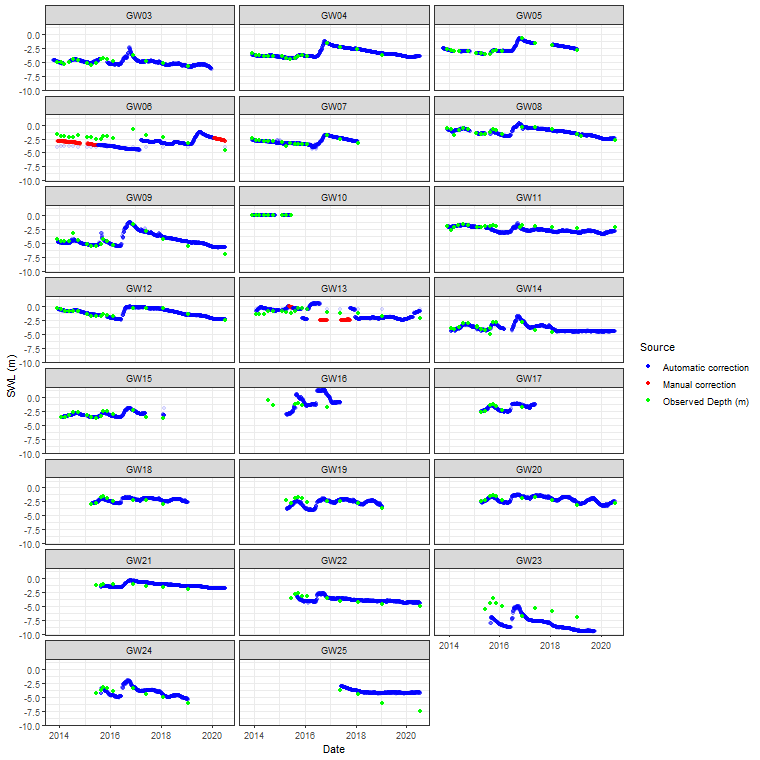
\includegraphics[width=1\linewidth]{../Figures/Final_Corrected_piezodepths} \caption{Overview of the corrected groundwater time series for all the wells}\label{fig:gw-series}
\end{figure}

Save the data to be used in the paper

\begin{Shaded}
\begin{Highlighting}[]
\FunctionTok{write\_csv}\NormalTok{(GW\_data\_output, }\StringTok{"../Data/Muttama\_Piezometer\_Output.csv"}\NormalTok{)}
\end{Highlighting}
\end{Shaded}


\end{document}
